\documentclass[11pt]{beamer}
\usepackage[T1]{fontenc}
\usepackage{lmodern}
\usepackage{tikz}
\usetikzlibrary{backgrounds,fit,calc,shadows,chains}
\usepackage{ocgx}
\usepackage{microtype}
\usepackage{url}

\tikzset{
  switch with mark/.style 2 args={
    path picture={
      \OCG{checkbox@#1}{
        \draw
        (path picture bounding box.south west)
        --
        (path picture bounding box.north east)
        (path picture bounding box.south east)
        --
        (path picture bounding box.north west)
        ;
      }
      \path let
      \p1 = (path picture bounding box.south west),
      \p2 = (path picture bounding box.north east),
      \p3 = (\x2-\x1,\y2-\y1)
      in
      (path picture bounding box.center)
      node[inner sep=0pt,anchor=center] {%\typeout{\x3-\y3}%
        \switchOCG{#2 checkbox@#1}{%
          \phantom{%
            \rule{\x3}{\y3}%
          }
        }};
      \typeout{switch with mark-#2-checkbox@#1}
    },
  },
  switch/.style={
    path picture={
      \path let
      \p1 = (path picture bounding box.south west),
      \p2 = (path picture bounding box.north east),
      \p3 = (\x2-\x1,\y2-\y1)
      in
      (path picture bounding box.center)
      node[inner sep=0pt,anchor=center] {%\typeout{\x3-\y3}%
        \switchOCG{#1}{%
          \phantom{%
            \rule{\x3}{\y3}%
          }%
        }};
      %\typeout{switch-#1}
    },
  },
  show/.style={
    path picture={
      \path let
      \p1 = (path picture bounding box.south west),
      \p2 = (path picture bounding box.north east),
      \p3 = (\x2-\x1,\y2-\y1)
      in
      (path picture bounding box.center)
      node[inner sep=0pt,anchor=center] {%\typeout{\x3-\y3}%
        \showOCG{#1}{%
          \phantom{%
            \rule{\x3}{\y3}%
          }%
        }};
      %\typeout{switch-#1}
    },
  },
  hide/.style={
    path picture={
      \path let
      \p1 = (path picture bounding box.south west),
      \p2 = (path picture bounding box.north east),
      \p3 = (\x2-\x1,\y2-\y1)
      in
      (path picture bounding box.center)
      node[inner sep=0pt,anchor=center] {%\typeout{\x3-\y3}%
        \hideOCG{#1}{%
          \phantom{%
            \rule{\x3}{\y3}%
          }%
        }};
      %\typeout{switch-#1}
    },
  },
  actions/.style n args={3}{
    path picture={
      \path let
      \p1 = (path picture bounding box.south west),
      \p2 = (path picture bounding box.north east),
      \p3 = (\x2-\x1,\y2-\y1)
      in
      (path picture bounding box.center)
      node[inner sep=0pt,anchor=center] {%\typeout{\x3-\y3}%
        \actionsOCG{#1}{#2}{#3}{%
          \phantom{%
            \rule{\x3}{\y3}%
          }%
        }};
      %\typeout{switch-#1}
    },
  },
}

\newcommand\TkzTileWallPaper[3]{
  \pgfmathtruncatemacro{\nx}{\paperwidth/#1}
  \foreach \dx in {0,...,\nx}{
    \pgfmathtruncatemacro{\ny}{\paperheight/#2}
    \foreach \dy in {0,...,\ny}{
      \node[anchor=south west,inner sep=0pt]
      at ([xshift=#1 * \dx,yshift=#2 * \dy]current page.south west)
      {\includegraphics[width=#1,height=#2]{#3}};
    }
  }
}

\setbeamersize{text margin left=3mm,text margin right=3mm}

\newcommand\latex{{\rmfamily\LaTeX}}

\begin{document}
\begin{frame}
  \frametitle{\latex,OCG \& Ti\emph{k}Z -- D�monstration}
  \framesubtitle{par Paul Gaborit avec l'aide de Paul Isambert}

  \def\mylist{red/0,yellow/60,green/120,cyan/180,blue/240,magenta/300}
  \centering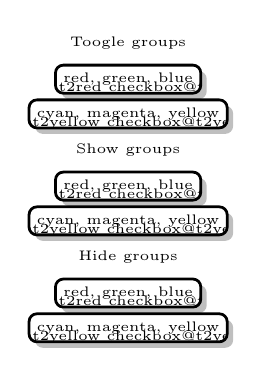
\begin{tikzpicture}[line width=1pt]
    \begin{scope}
      \foreach \col/\angle in \mylist
      {
        \colorlet{rgb \col}[rgb]{\col}
        \draw  (\angle:5mm) circle [radius=10mm];
        \begin{pgfonlayer}{background}
          \OCG{t1\col}{
            \fill[fill=rgb \col,fill opacity=.5]
            (\angle:5mm) circle [radius=10mm];
          }
        \end{pgfonlayer}
        
        % \begin{pgfonlayer}{background}
        \node[rounded corners=1mm,draw,line width=1pt,
        minimum size=3mm,fill=rgb \col,fill opacity=.5,
        drop shadow,
        switch with mark={t1\col}{t1\col}]
        at (\angle:20mm){};
        % \end{pgfonlayer}
      }
    \end{scope}
    \begin{scope}[xshift=70mm]
      \foreach \col/\angle in \mylist
      {
        \colorlet{cmy \col}[cmyk]{\col}
        \draw  (\angle:5mm) circle [radius=10mm];
        \begin{pgfonlayer}{background}
          \OCG{t2\col}{
            \fill[fill=cmy \col,fill opacity=.5]
            (\angle:5mm) circle [radius=10mm];
          }
        \end{pgfonlayer}
        \node[rounded corners=1mm,draw,line width=1pt,
        minimum size=3mm,fill=cmy \col,fill opacity=.5,
        drop shadow,
        switch with mark={t2\col}{t2\col}]
        at (\angle:20mm){};
      }
    \end{scope}

    \begin{scope}%
      [xshift=35mm,start chain=going below,node distance=.5mm,font=\tiny]
      \node[on chain] at (0,20mm) {Toogle groups};
      \node%
      [on chain,draw,rounded corners=1mm,fill=white,drop shadow,
      minimum size=3mm,inner sep=1mm,
      switch={%
        t1red checkbox@t1red %
        t1blue checkbox@t1blue %
        t1green checkbox@t1green %
        t2red checkbox@t2red %
        t2blue checkbox@t2blue %
        t2green checkbox@t2green%
      },
      ]
      {red, green, blue};
      \node%
      [on chain,draw,rounded corners=1mm,fill=white,drop shadow,
      minimum size=3mm,inner sep=1mm,
      switch={%
        t1yellow checkbox@t1yellow %
        t1cyan checkbox@t1cyan %
        t1magenta checkbox@t1magenta %
        t2yellow checkbox@t2yellow %
        t2cyan checkbox@t2cyan %
        t2magenta checkbox@t2magenta%
      },
      ]
      {cyan, magenta, yellow};

      \node[on chain] {Show groups};
      \node%
      [on chain,draw,rounded corners=1mm,fill=white,drop shadow,
      minimum size=3mm,inner sep=1mm,
      show={%
        t1red checkbox@t1red %
        t1blue checkbox@t1blue %
        t1green checkbox@t1green %
        t2red checkbox@t2red %
        t2blue checkbox@t2blue %
        t2green checkbox@t2green%
      },
      ]
      {red, green, blue};
      \node%
      [on chain,draw,rounded corners=1mm,fill=white,drop shadow,
      minimum size=3mm,inner sep=1mm,
      show={%
        t1yellow checkbox@t1yellow %
        t1cyan checkbox@t1cyan %
        t1magenta checkbox@t1magenta %
        t2yellow checkbox@t2yellow %
        t2cyan checkbox@t2cyan %
        t2magenta checkbox@t2magenta%
      },
      ]
      {cyan, magenta, yellow};

      \node[on chain] {Hide groups};
      \node%
      [on chain,draw,rounded corners=1mm,fill=white,drop shadow,
      minimum size=3mm,inner sep=1mm,
      hide={%
        t1red checkbox@t1red %
        t1blue checkbox@t1blue %
        t1green checkbox@t1green %
        t2red checkbox@t2red %
        t2blue checkbox@t2blue %
        t2green checkbox@t2green%
      },
      ]
      {red, green, blue};
      \node%
      [on chain,draw,rounded corners=1mm,fill=white,drop shadow,
      minimum size=3mm,inner sep=1mm,
      hide={%
        t1yellow checkbox@t1yellow %
        t1cyan checkbox@t1cyan %
        t1magenta checkbox@t1magenta %
        t2yellow checkbox@t2yellow %
        t2cyan checkbox@t2cyan %
        t2magenta checkbox@t2magenta%
      },
      ]
      {cyan, magenta, yellow};
    \end{scope}
    
  \end{tikzpicture}\par

\end{frame}

\foreach \name/\link/\ltxlink/\tiles in {%
  The Big Show/%
  {http://designfestival.com/the-cicada-principle-and-why-it-matters-to-web-designers/}/%
  {http://latex-community.org/know-how/433-tiled-backgrounds}/%
  {%
    curtain1/32.7pt/\paperheight,%
    curtain2/90pt/\paperheight,%
    curtain3/210.9pt/\paperheight%
  },%
  Mosaic/%
  {http://designfestival.com/cicada/break-it-down/?id=95}/%
  {http://latex-community.org/know-how/433-tiled-backgrounds}/%
  {%
    mosaic1/30pt/30pt,%
    mosaic2/70pt/70pt,%
    mosaic3/110pt/110pt,%
    mosaic4/110pt/110pt%
  }%
}{
  \begin{frame}
    \begin{tikzpicture}[remember picture,overlay]
      \foreach \pictname/\wid/\hei in \tiles {
        \OCG{\pictname}{\TkzTileWallPaper{\wid}{\hei}{\pictname}}
      }

    \end{tikzpicture}
    
    \centering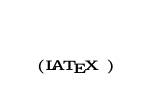
\begin{tikzpicture}[start chain=going below,node distance=1em]
      \node[fill=white,fill opacity=.75,align=center,
      text=black,font=\tiny\bfseries,text opacity=1,
      on chain,
      rounded corners=2mm]
      {{\huge\name}\\\url{\link}\\(\latex{} \url{\ltxlink})};
      \foreach \pictname/\wid/\hei in \tiles {
        \node[on chain,text=white,fill=black,fill opacity=.5,text opacity=1,
        text width=3cm,align=center,font=\bfseries]
        (a)
        {\hspace{5mm}\pictname};
        \node[rounded corners=1mm,draw,line width=1pt,%
        minimum size=3mm,top color=white,bottom color=black,
        fill opacity=.5,
        drop shadow={fill=black},
        switch with mark={\pictname}{\pictname}]
        at ([xshift=3mm,yshift=.5mm]a.west) {};
        
      }
    \end{tikzpicture}\par
  \end{frame}
}

\begin{frame}
  \frametitle{Microtype demo}

  \def\sampletext{%
    Margin kerning is the adjustments of the characters at the
    margins of a typeset text.  A simplified employment of margin
    kerning is hanging punctuation. Margin kerning is needed for
    optical alignment of the margins of a typeset text, because
    mechanical justification of the margins makes them look rather
    ragged. Some characters can make a line appear shorter to the
    human eye than others. Shifting such characters by an
    appropriate amount into the margins would greatly improve the
    appearance of a typeset text.%
  }

  \tikzset{
    checkbox/.style={
      rounded corners=1mm,draw,line width=1pt,%
      minimum size=3mm,top color=white,bottom color=black,
      fill opacity=.5,
      drop shadow={fill=black},
    },
    sampletext/.style={
      text width=8cm,align=justify,
      font=\small,
      fill=black!5,
      inner xsep=1.5cm,
      inner ysep=1cm,
      draw=gray,
    },
  }

  {\centering
    \begin{tikzpicture}
      \OCG{withprotrusion}{
        \microtypesetup{protrusion=true}%
        \OCG{withexpansion1}{%
          \microtypesetup{expansion=true}%
          \node[sampletext]{\sampletext\par};%
        }
        
        \OCG*{withoutexpansion1}{%
          \microtypesetup{expansion=false}%
          \node[sampletext]{\sampletext\par};%
        }
      }
      
      \OCG*{withoutprotrusion}{
        \microtypesetup{protrusion=false}%
        \OCG{withexpansion2}{%
          \microtypesetup{expansion=true}%
          \node[sampletext]{\sampletext\par};%
        }
        
        \OCG*{withoutexpansion2}{%
          \microtypesetup{expansion=false}%
          \node[sampletext]{\sampletext\par};%
        }
      }
    \end{tikzpicture}\par
  }

  Microtype :
  \begin{tikzpicture}
    \node[checkbox,
    switch with mark={protrusion}{withprotrusion withoutprotrusion}]
    {};
  \end{tikzpicture} protrusion 
  \begin{tikzpicture}
    \node[checkbox,
    switch with mark={expansion}%
    {withexpansion1 withoutexpansion1 withexpansion2 withoutexpansion2}]
    {};
  \end{tikzpicture} expansion
  
\end{frame}

\end{document}
%%% Local Variables: 
%%% mode: latex
%%% TeX-master: t
%%% End: 
